\documentclass[10pt,conference,compsocconf]{IEEEtran}
\usepackage[T1]{fontenc}
\usepackage[utf8]{inputenc}
\usepackage{url}
\usepackage{comment}
\usepackage{graphicx}
\usepackage{multirow}
\usepackage{booktabs}
\usepackage{amsmath}

\usepackage{tikz}
\usetikzlibrary{fit}

\usepackage{acronym}
\acrodef{iaas}[IaaS]{Infrastructure as a Service}
\acrodef{SaaS}{Software as a Service}
\acrodef{PaaS}{Platform as a Service}
\acrodef{dag}[DAG]{directed acyclic graph}
\acrodef{vm}[VM]{Virtual Machine}
\acrodef{pm}[PM]{Physical Machine}
\acrodef{btu}[BTU]{billing time unit}
\acrodef{EC2CU}{EC2 Compute Unit}
\acrodef{HPC}{High Performance Computing}
\acrodef{unistra}{University of Strasbourg}
\acrodef{rv}[RV]{random variable}
\acrodef{pdf}[PDF]{probability density function}
\acrodef{cdf}[CDF]{cumulative distribution function}
\acrodef{mcs}[MCS]{Monte-Carlo simulation}
\acrodefplural{mcs}[MCS's]{Monte-Carlo simulations}
\acrodef{des}[DES]{discrete event simulation}
\acrodef{ci}[CI]{confidence interval}

\newcommand*\rot{\rotatebox{90}}
\newcommand{\pmpc}[1]{$\pm#1\%$}
\newcommand{\etal}[1]{\emph{#1 et al.}}
\newcommand{\pc}[1]{$#1\%$}

%\let\OLDthebibliography\thebibliography
%\renewcommand\thebibliography[1]{
%  \OLDthebibliography{#1}
%  \setlength{\parskip}{0pt}
%  \setlength{\itemsep}{5pt plus 0.5ex}
%}

%\IEEEtriggeratref{15}

%\title{Modeling the accuracy of Monte-Carlo approach for Cloud based workflow
%  simulations.}
%\title{Executing Batch Jobs on Clouds: How to Predict Reality Accurately?}
\title{Improving Cloud Simulation using the Monte-Carlo Method}


\author{\IEEEauthorblockN{Luke~Bertot 
			and Stéphane~Genaud 
			and Julien~Gossa}
	\IEEEauthorblockA{Icube-ICPS --- UMR 7357, Univeristé de Strasbourg, CNRS\\
		P\^ole API Blvd S. Bant, 67400 Illkirch-Graffenstaden\\
		email: \url{lbertot@unistra.fr}, \url{genaud@unistra.fr}, \url{gossa@unistra.fr}}
	}



\begin{document}

\maketitle

\begin{abstract}
  In the  cloud computing  model, cloud providers  invoice clients  for resource
  consumption. Hence, tools helping the client to budget the cost of running
  their application are  of pre-eminent  importance. However, the opaque and
  multi-tenant nature of clouds, make job runtimes both variable and hard to
  predict.  In this  paper, we  propose an improved simulation framework that
  takes into account  this variability using the Monte-Carlo method.

  We consider  the execution of batch jobs on  an actual platform, scheduled
  using typical  heuristics based  on the  user estimates  of tasks' runtimes. We
  model  the observed  variability through  simple  distributions to use  as
  inputs  to the  Monte-Carlo  simulation. We show that, our method can capture 
  over  90\% of the empirical observations of total execution times.
\end{abstract}

\begin{IEEEkeywords}
cloud computing, computer simulation, monte carlo methods.
\end{IEEEkeywords}

%\tableofcontents

\section{Introduction.}

\subsection{Simulation}

Because they allow one to experiment without having to build or even use a real 
platform, simulations are a cornerstone of the study of distributed
systems and clouds.  
Most cloud simulators  are based on \ac{des}. Given a set of inputs a \ac{des}
produces deterministic output results by computing the timeline of the events
generated by the inputs.  In this paper
we simulate task \acp{dag}, based on task runtime as input in order get the total
execution time, \emph{makespan}, and the execution cost.

However, when the simulated system is subject to variability, it is difficult
to establish  the  validity of  simulation  results formally. Indeed, given some
defined inputs, a DES outputs a single deterministic result, while a real system
will output  slightly different results for each repeated execution.

\subsection{Stochastic Simulation and Monte-Carlo Method}

\label{sc:relwork-stochastic}
For  more   comprehensive  predictions  in  such   variable  environments,  the
simulation must  be \emph{stochastic}.  In stochastic simulations  inputs become
distributions of possible runtimes, provided as \acp{rv}.
The  result  of one  such  simulation  is  itself  a distribution of the
possible results.

Numerical methods have been proposed for solving stochastic
\acp{dag}~\cite{Li97,Ludwig01}. However, they are computationally intensive and
their core constraint, the independence of \acp{rv}, can not always be
guaranteed. 

On the other hand, a \ac{mcs}, depicted in Figure~\ref{fig:mc-process}, samples
the possible outcomes by testing  multiple \emph{realizations} in a
deterministic fashion.  Each realization is a possible scenario obtained by
drawing a runtime from each task's respective \ac{rv}.  Realizations are then
simulated using traditional methods like \ac{des}.  Eventually, given enough
realizations, the distribution of the simulation results will  tend towards the
distribution of the equivalent stochastic simulation. 

\section{Work Context}
\label{sec:work-context}
\begin{figure}
	\centering
	\resizebox{0.9\linewidth}{!}{%
		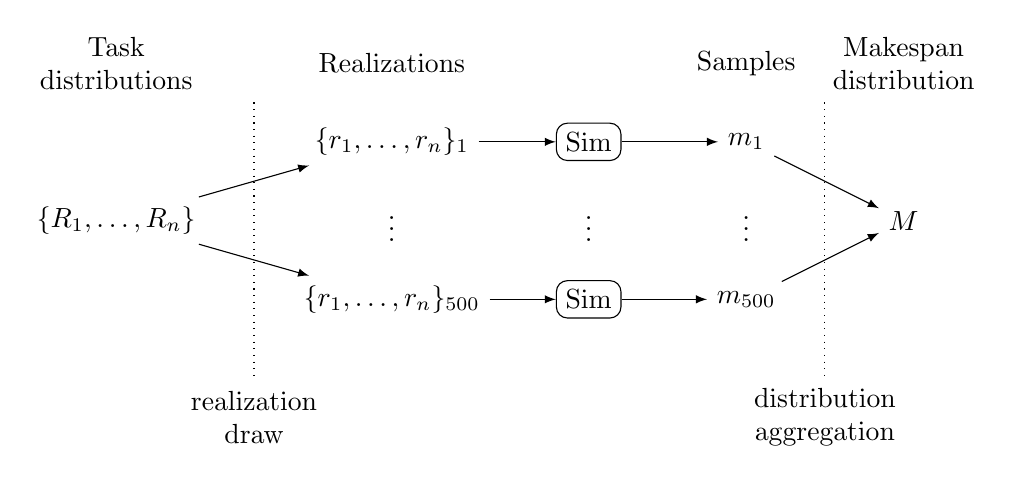
\begin{tikzpicture}[
sim/.style={%
draw, 
rounded corners
}
]
%% Origin node
\node[align=center]at(0,2){Task\\distributions};
\node at(0,0)(orig){$\{R_1,\ldots,R_n\}$};
%% Realisations
\node at(3.5,2){Realizations};
\node[]at(3.5,1)(pert1){$\{r_1,\ldots,r_n\}_1$};
\node at(3.5,0){\vdots};
\node at(3.5,-1)(pert5){$\{r_1,\ldots,r_n\}_{500}$};
\draw[-{latex}](orig)--(pert1);
\draw[-{latex}](orig)--(pert5);
%%
\node[sim]at(6,1)(s1){Sim};
\node[sim]at(6,-1)(s5){Sim};
\node at(6,0){\vdots};
\draw[-{latex}](pert1)--(s1);
\draw[-{latex}](pert5)--(s5);
%% Makespans
\node at(8,2){Samples};
\node at(8,1)(M1){$m_1$};
\node at(8,-1)(M5){$m_{500}$};
\node at(8,-0){\vdots};
\draw[-{latex}](s1)--(M1);
\draw[-{latex}](s5)--(M5);
%% Consolidation
\node[align=center]at(10,2){Makespan\\distribution};
\node at(10,0)(r){$M$};
\draw[-{latex}](M1)--(r);
\draw[-{latex}](M5)--(r);
%%phases
\node[align=center]at(1.75,-2.5)(df){realization\\draw};
\draw[dotted](1.75,1.5)--(1.75,-2);
\node[align=center]at(9,-2.5)(df){distribution\\aggregation};
\draw[dotted](9,1.5)--(9,-2);
\end{tikzpicture}

		}
\caption{Overview of a Monte-Carlo simulation~: $500$ realizations are generated
	by drawing runtimes ($r_t$) for each of the $n$ tasks provided
	distributions ($R_t$); every realization is then simulated; the 
	resulting makespan samples make up the final result M.}\label{fig:mc-process}
\end{figure}

The  study conducted  in this  paper  is built upon a genuine comparison  between
experiments  run in  actual environments  and experimental  results obtained  by
simulation.  

\subsection{Real Execution Setup}
Using the Schlouder~\cite{Michon17} cloud batch-scheduler, we carried out
multiple executions of a scientific application, OMSSA~\cite{Geer2004} on a
private cloud.
The application was scheduled 200 times favoring alternatively low runtimes (ASAP) or 
low cost (AFAP). These executions were performed on an Openstack 96-core cloud. 

\subsection{Simulated Execution Setup}
Using the SimGrid~\cite{simgrid} simulation framework we built a simulator
capable of simulating our cloud platform, scheduling, and executions. This
simulator has been fine-tuned against the real execution traces, and is precise
to the second for executions performed by Schlouder. This \ac{des} outputs the
makespan, in seconds, and the cost, in \emph{BTU} (\emph{billing time unit},
e.g. VM$\times$hour) for the simulated execution.

\section{Enriched Simulation Framework}\label{sec:enriched-sim}

\subsection{Simulation process}


As depicted in Figure~\ref{fig:mc-process} the \ac{mcs} consists in repeatedly
drawing runtimes for each task, to form realizations. Each realization is then
simulated independently and the resulting makespans, the total runtime of the
application, are aggregated in a distribution. 

\subsection{Input Modeling}\label{sec:im}
The \ac{mcs} requires a runtime distribution for every task. Although more
precise input distributions will always yield more precise results we aim to
show that even simple models will provide sufficiently accurate simulation
results. In our model, the tasks runtimes follow a uniform distribution centered
on the average expected runtime for a given task $t$ ($\bar{r_t}$). The relative
spread of each distribution represents the expected platform variability and is
called the perturbation level ($P$). As such the distribution of possible 
runtimes for a task $t$,  $R_t$ is expressed as :
\begin{equation}
	R_t=\mathcal{U}(\bar{r_t}\cdot{}(1-P), \bar{r_t}\cdot{}(1+P)) 
\end{equation}
We computed the expected variability of our platform as being the average across
all tasks of the worst-case deviation from the expected value for each task. The
perturbation level given by this method is $P\approx{}10\%$ for both strategies.

% Using a similar metric,\cite{pics} also 
%observed most deviations to be within 10\% of the average runtime when working
%on Amazon EC2 instances with dedicated CPUs.

\section{Evaluation}
\label{sec:eval}
Using this model,  we ran a 500-iteration \ac{mcs} for each strategy.
The  resulting distributions are  shown  in  Figure~\ref{fig:fit}. 
The makespan  density  graph  shows the simulation  result  distribution as
filled  curves and the  real  observed executions as non-filled 
curves. On the \acused{btu}\ac{btu} count graph, the left bar represents
the empirical data, and the right  bar the prediction from the simulation. 

The distribution  of simulated makespans covers fairly  well the
ranges of  observed makespans, notwithstanding a  slight right skew and shift of
the empirical makespan distribution. Likewise the range of BTU numbers required 
for an execution is correct but the simulated distribution differs slightly. The
divergence between the simulated and observed distribution is due to our
simplified model described in section~\ref{sec:im}. We quantify this divergence
by fitting the simulated distribution to a Normal distribution, and producing
\ac{ci}. The 95\%\ac{ci} captures 90\% of real executions in ASAP and 92\% in
AFAP. Using the 99\%\ac{ci} yields capture rates of 98\% and 100\% respectively.

\begin{figure}
	\center
	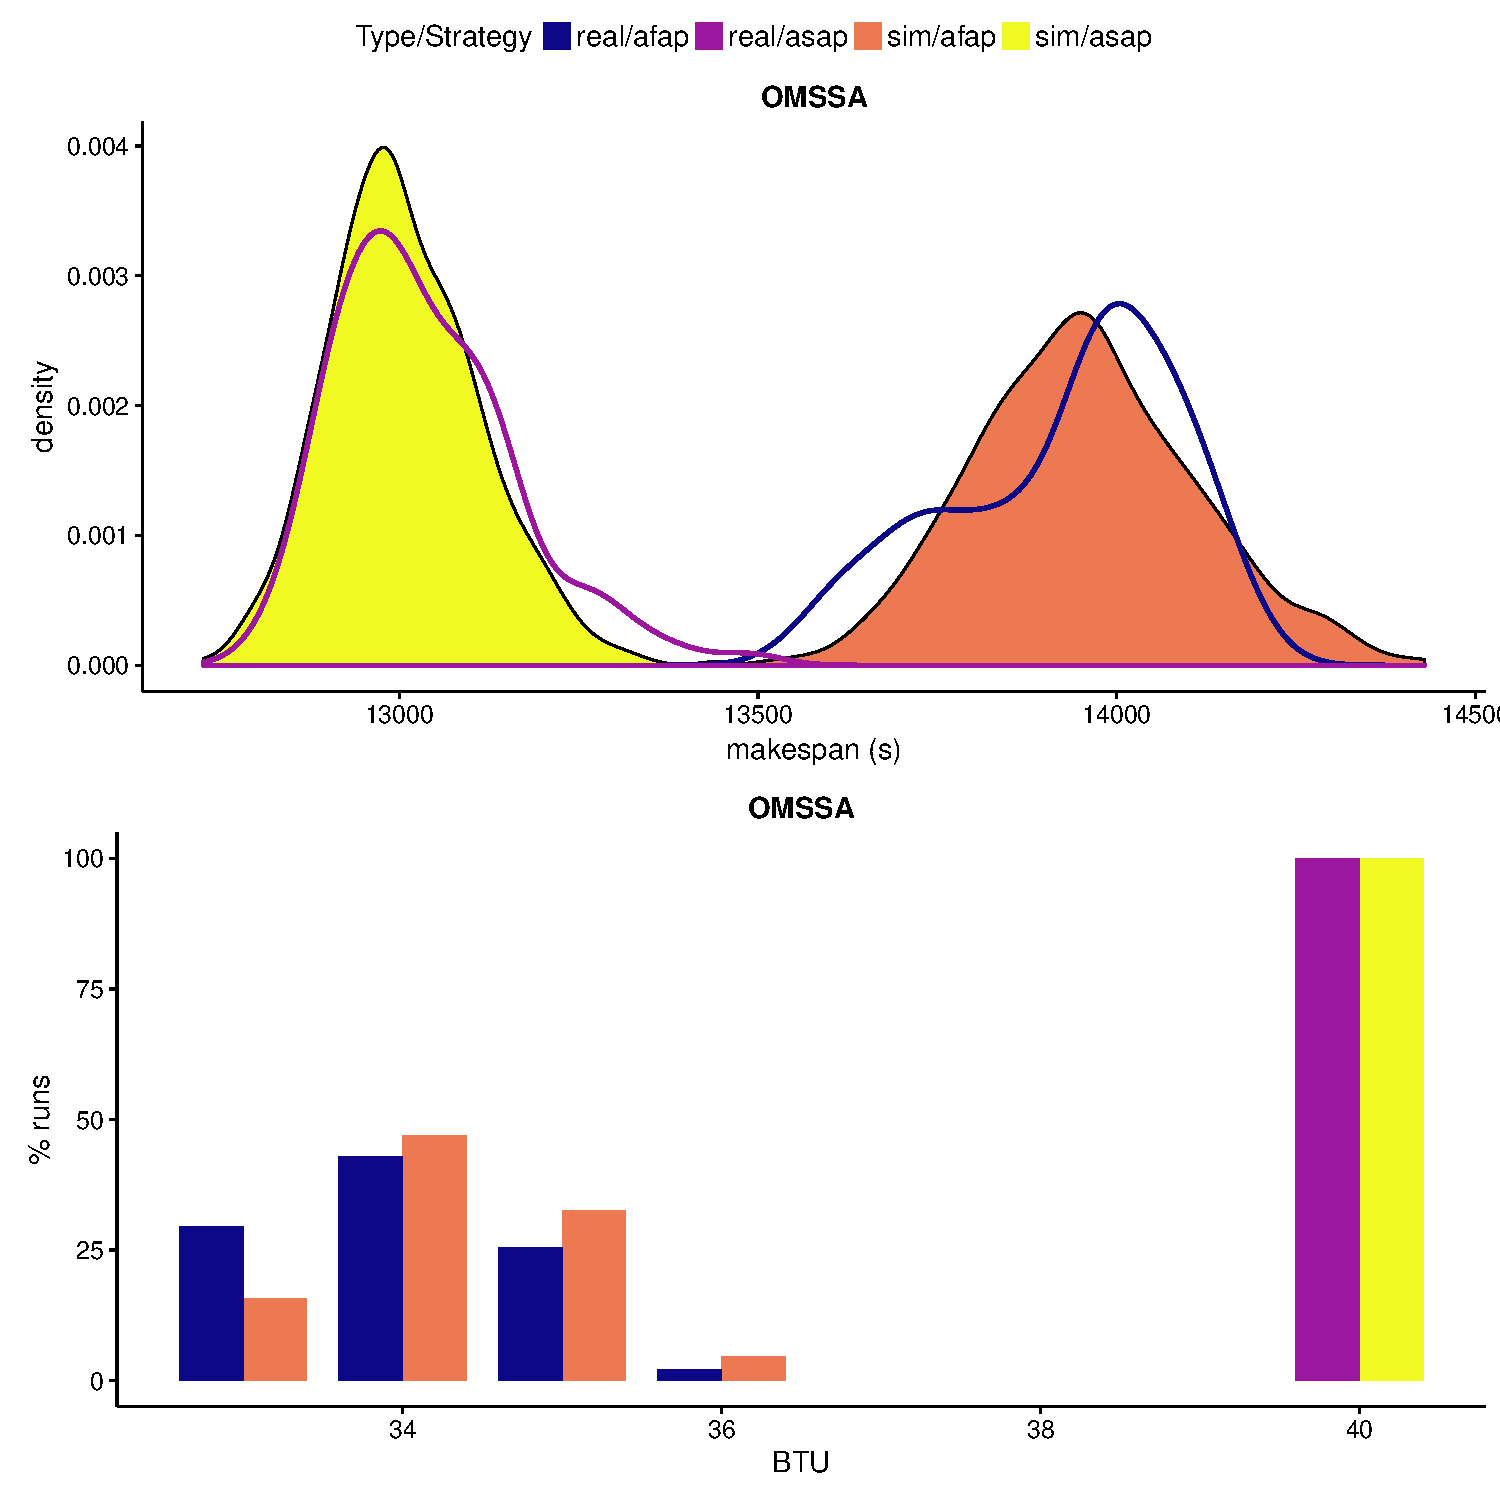
\includegraphics[width=1.0\linewidth]{gfx/PP_fit.pdf}
	\caption[caption]{Makespan and BTU count distribution for OMSSA Monte
	  Carlo Simulation compared to reality at 10\% perturbation level.\\ 
	  \textit{Reading example: Simulating AFAP with OMSSA leads to makespans 
	  roughly ranging from 12800 s to 13400 s and BTU counts ranging from 33 to 36.}
	}
	\label{fig:fit}
\end{figure}

\section{Conclusion}
In this paper, we propose a \acl{mcs} extension  to a  discrete  event  simulator based  on
SimGrid.  This  extension provides stochastic predictions which are more
informative than single values produced by
traditional discrete  event simulators. In this work we show that the
variability we seek to account for can be modeled  by a  single parameter,
called the perturbation  level and applied  to all task runtimes. We apply
our method in  a real setting, for which we have collected  execution traces.  
In light of  these empirical observations, our study shows that the
proposed method could capture over 90\% of the observed makespans given  an
appropriate perturbation  level.

\bibliographystyle{IEEEtran}
\bibliography{montecarlo-simulation}

\end{document}
% vim:spell spelllang=en:
